
\documentclass[12pt,oneside,a4paper]{article}
%
\usepackage{graphicx}
\usepackage{tabularx}
\usepackage{url}
\usepackage[latin1]{inputenc}
%\usepackage[utf8]{inputenc}
\usepackage[left]{eurosym} 
\usepackage{times}
\usepackage{pdfpages}
\usepackage{todonotes}
\usepackage{enumerate}

% We don't want a special font for urls (looks bad with times):
\urlstyle{same}

% Graphics extensions and path:
%\DeclareGraphicsExtensions{.pdf,.png,.jpg}
%\DeclareGraphicsExtensions{.eps,.ps}
%\graphicspath{{figures/}}

%
% Page size
%
\usepackage[top=25mm,left=25mm,right=25mm,bottom=25mm]{geometry}

\setlength{\headheight}{15pt}    % Necessary to avoid fancyhdr warning.


\newcommand\LongTitle{Humidity, clouds and snow in the Arctic}
\newcommand\ShortTitle{Humidity, clouds and snow in the Arctic}



%
% Heading
%
\newcommand{\pagevers}[2]{
\ifnum\thepage=1 
#1
\else#2
\fi
}
%
\usepackage{fancyhdr}
\pagestyle{fancy}
\chead{}
%\rhead{\pagevers{}{\bf \thepage}}
\rhead{\thepage}
\rfoot{\small \it \ShortTitle\ ---\  Application to SNSA 2021-R}
\cfoot{}
\lfoot{}
%\renewcommand{\headrulewidth}{\pagevers{0pt}{0.2pt}}
\renewcommand{\headrulewidth}{0.2pt}
\renewcommand{\footrulewidth}{0pt}


\newcommand{\docname}[1]{\lhead{\small #1}}

%
% Section titles
%
\usepackage[small]{titlesec}
\titlespacing*{\section}{0pt}{*3.3}{*0.5}
%
% 
%
\def\compactitems{\parskip0pt\topsep0pt\partopsep0pt\parsep0pt\itemsep0pt}

% Struts for better table formatting:
\newcommand\T{\rule{0pt}{2.6ex}}
\newcommand\B{\rule[-1.2ex]{0pt}{0pt}}


\newcommand{\FIXME}[1]{{\bfseries \textcolor{red}{FIXME:} #1}}
\newcommand{\md}[1]{\mbox{#1-d}}
%\newcommand{\3d}{3d}

%\hyphenation{3-d}
\uchyph=0

%%% Local Variables: 
%%% mode: latex
%%% TeX-master: t
%%% End: 



\docname{Project description}
\usepackage{graphicx}
\usepackage{caption}
\usepackage{subcaption}
\usepackage{multirow}
\usepackage{amsmath}
\captionsetup[figure]{font=normalsize,labelfont=normalsize}

%
% References
%
\usepackage{natbib}
\bibliographystyle{agu04}     
\setlength{\bibsep}{0mm}


\newcommand\wpstart[3]{\noindent\textbf{WP #1, #2}\hspace{\stretch{1}}Priority #3%
	\vspace{-4mm}\\\rule{\textwidth}{0.5pt}\\}
\newcommand\wpenda[4]{%
	\noindent -----\\ 
	\begin{tabularx}{0.95\hsize}{l p{133mm}}    
		\hspace*{-1.1ex}Start\,--\,end: & #1\\
		\hspace*{-1.1ex}Main output: & #2\\
		\hspace*{-1.1ex}Main risks: & #3\\
	\end{tabularx}\\
	\vspace{-2.2ex}\noindent\rule{\textwidth}{0.5pt}\\
}


\begin{document}
	
	
	\thispagestyle{empty}
	\vspace*{-10mm}
	\noindent
	\textbf{\Large \LongTitle}




\section{General summary}
%
The Arctic is a water world, experiencing rapid warming. Passive microwave 
satellite observations are in general required to study water in the region and
the basic aim of the project is to improve the utilisation of this data source,
particularly the high-frequency part. The project targets water in the
atmosphere. The primary concern is the estimation of humidity, but the retrieval
system is highly versatile and retrievals of liquid water content, snowfall and
sea-ice concentration (in order of priority) are also feasible.

We propose a physically-based, Bayesian-oriented, machine-learning model for
the task. The model is trained by detailed 3D radiative transfer simulations,
to generate local scenes of measured radiances. The input to the simulations
has a horizontal resolution finer than the size of the satellite footprints.
For example, high-resolution SAR imagery is applied to describe the
distribution of sea-ice\,/\,open water at a resolution of ?\,km. As a result,
aspects like inhomogeneous filling and overlap of the footprints are
incorporated into the simulations and are then automatically included in the
retrieval process, in contrast to existing data extraction. Precipitation and
clouds are modelled in detail by combining a mesoscale model with an in-house
expertise on microwave radiative transfer involving hydrometeors. As we cover
all significant parts of the ``forward problem'', our inversions can be truly
``all-sky''; we aim for a zero data rejection (for the set of channels
considered).

The resulting dataset(s) would play an important role in not only analysing the
variability of water above the Arctic, but also in deciphering the
ongoing trends involved in the Arctic amplification of global warming.



%Water vapour plays an important role in the water and energy cycle over the polar regions, especially over Arctic. Over the Arctic, changes in the water vapour content are most sought to observe the warming trends, also know and Artic amplification. However over poles, the ground measurements are sparse and the performance of the satellite retrievals is constrained by the highly variable surface emissivity. The basic aim of this project is to develop new retrieval algorithms principally for total water vapour (TWV) from satellite microwave radiometer data over the Arctic. We propose a physically based retrievals, using a Bayesian machine learning based inversion method. Additionally, this algorithm could be used to also retrieve side products like total liquid water content (LWC) and sea-ice concentration (SIC). A key feature of this algorithm would be the use high resolution SAR imagery to classify sea-ice and open waters. Fine scale sea-ice information is necessary for distinguishing emissivity between different surface types. Another crucial aspect of the development line will be to use data from multiple microwave frequencies, with different footprint size, and avoiding the remapping of data. The overall scheme shall be similar to the one in a parallel SNSA 2021 proposal submitted by co-applicant Patrick Eriksson.
%The resulting dataset would play an important role in not only analysing the water vapour variability of the Arctic atmospheric but also in deciphering the trends the Arctic climate change.


\subsection{Background}
%
\label{sec:background}
Some info from Luisa (1/2 page)

\subsection{Previous work}
%
\label{sec:previousworks}
%
Ground-based measurements inside the Artic region are very sparse and can not
be used for monitoring, but are still of interest for validation purpose.
Hence, we must rely on satellite data. As the area experiences polar night and
has extensive cloud cover, optical and infrared techniques suffer basic
limitations that microwave radiometry lacks and the later is the set of
satellite sensors of concern here. Over the polar regions, a challenge
encountered by passive microwave observations is the high and highly variable
contribution by surface emission. 

The most important work towards retrieval of WVP from microwave humidity sounders (such as Advanced Microwave Sounding Unit-B (AMSU-B) and Microwave
Humidity Sounder (MHS)) comes from University of Bremen. Their retrieval
concept was initiated by \citet{miao:2001:atmos}, where they utilized water
vapour absorption channels around 183\,GHz and 150\,GHz window channel to
retrieve total water vapour (TWV) upto 7\,kg m$^{-2}$. Subsequently in the
study \citep{} they extended this approach to include 89\,GHz to retrieve TWV
upto 15\,kg m$^{-2}$ over sea-ice regions and formulated a relationship between
sea-ice emissivity over different frequencies using measurement campaigns.
Later, \cite{scarlat:2018:retri} extended the method to include all surface
types using AMSU-B. A comparison of the retrieved WVP against ERA-Interim
showed that the over winter months, the RMSD was 1.86\,kg m$^{-2}$ but over
summer months the errors were up to 5.67\,kg m$^{-2}$ due to the algorithm being
constrained by its upper retrieval limit of 15\,kg m$^{-2}$. Besides MW sounding,
an attempt at TWV has also been made using low frequency microwave observations
from Advanced Microwave Scanning Radiometer (AMSR). For example,
\citet{scarlat:2017:exper} use optimal estimation (OEM) for multi-parameter
retrieval over Arctic, and \citet{zabolotskikh:2020:anadv} attempt at TWV
retrieval over both open ocean and sea-ice regions using neural networks based
inversion. In both products, the highest uncertainties in the retrieval are
linked to the empirical estimates of surface emissivity over sea-ice regions. Infact the skill of all available satellite based WV retrievals in this region is highly variable over different atmospheric and surface conditions. For example, in central Arctic, the differences between monthly means over summer months can be as high as 30\% \citep{crewell:2021:asyst}.
 
The lack of an accurate atmospheric data over the extensive Arctic sea-ice regions has implications in the forecast skill of numerical weather prediction (NWP) models. Though the  models are themselves suffer from limitations associated with the modelling of snow, sea ice, mixed-phase clouds, \citet{lawrence:2019:usean} show that MW sounding observations have a clear positive impact on the predictive skill in the summer months. Over the winter months the optimal utilisation of the observations is constrained by the presence of snow and sea-ice. Infact,  increasing the usage of satellite data over all surfaces in Integrated Forecast System (IFS) is identified as one of the priorities in ECMWF Strategy for 2021-2030. 


\subsection{The way forward : Problems and solutions }

%\subsubsection{Problems and solutions}

Remote sensing provides indirect measurements and the data retrieval always
offers some degree of complexity. When using passive satellite microwave data
to estimate humidities over the Arctic region, as mentioned, the main
limiting factor is the surface's contribution to measured radiances. The
special role of the surface is due to high atmospheric transmissivities and the
difficulties to predict the surface properties of snow (on either land or ice).
The main solution today is to reject channels with a significant surface
contribution. This gives a low utilisation rate of the satellite data, and
leaves the humidity close to the surface unconstrained.

For this reason, efforts are being made to improve the "forward modelling",
i.e.\ use auxiliary data to predict the local radiative properties of snow and sea-ice \citep[e.g.][]{tonboe:2010:thesi}. This constitutes a very hard problem as the properties depend on a high number of realistic snow and sea-ice variables. There will be progress in the area, but it will likely be slow. There is also another, less discussed, consideration, that the satellite footprint can cover both sea ice and open water. To handle this, a large scale ice-fraction is not sufficient, even the distribution of ice and water inside the footprint matters. That is, retrievals above leads are particularly
problematic. The risk of having an inhomogeneous footprint increases with
footprint size, and good spatial resolution is thus advantageous even if the
atmospheric fields show little horizontal variability.



We will attack these issues from a new angle, now feasible due to progress in
machine learning (ML). We avoid the limitations in traditional approaches by
basing the inversions on a retrieval database, that is used to train the ML
model. The simulated observations in the database are generated on
high-resolution data and variations of both surface and atmospheric variables
inside the footprint get included. In addition, by simulating "scenes" of
adjacent footprints, and not just individual ones, the information hidden in
the overlap of footprints can be exploited. The later effectively increases the
horizontal resolution, but also provides background spatial information, such
as indications on if the surface is homogeneous or mixed.

% IK-  moved this section as part of 2.1
%\subsubsection{Some clarifications}

%The ML approach to be applied is introduced by us and operates in a Bayesian manner. Most importantly, it provides robust case specific error estimates. That is, an uncertainty is assigned to each individual retrieval.

%The database works like the prior assumptions in a standard Bayesian retrieval, but by using ML we are not restricted to Gaussian statistics, can handle strongly non-linear problems, and we can include aspects that are very difficult to handle in traditional retrievals (such as inhomogeneuos footprints). It is not needed to predict the conditions exactly where the observation is made, it suffices that simulations have a similar variability as reality. The ML algorithm uses the database provided to give the posterior knowledge of the quantity sought, given the scene of observations.

%If useful additional information can be provided, this can be incorporated in the ML training. For example, if there is progress in snow modelling and the local emissivity can be estimated with some certainty, this can be seen as a virtual measurement and be used to improve the ML model.

\section{Project description}
%
\subsection{Scientific objectives and considerations}
The main objective of this study is to provide physical standalone water retrievals over the Arctic from microwave instruments, which can be comparable to or better in performance than existing reanalyses and satellite based products. The idea would be to combine a database based on sophisticated 3D radiative transfer with ML to solve the Arctic water retrieval and estimate the associated uncertainties. The primary task would be to estimate humidity, however, a simultaneous retrieval of liquid water content would also be undertaken as a second priority.
Nonetheless, before going ahead, it is crucial to elucidate the following:
\begin{itemize}
\item  The retrieval database will work like the prior assumptions in a standard Bayesian retrieval, but by using ML we will not be restricted to Gaussian statistics. ML can handle strong non-linear problems, and we can include aspects that are very difficult to handle in traditional retrievals (such as inhomogeneous footprints). It is not needed to predict the conditions exactly where the observation is made, it is sufficient for the simulations to have a similar variability as reality. The ML algorithm uses the database provided to give the posterior knowledge of the quantity sought, given the scene of observations.
\item  If useful additional information is available during the course of the project, it can be incorporated into the ML training. For example, if there is progress in snow modelling and the local emissivity can be estimated with some certainty, this can be seen as a virtual measurement and be used to improve the ML model. 
\end{itemize}

\subsection{Data and tools}
% 
\subsubsection{Satellite instruments}

The scheme developed here would not only be applicable to existing conical radiometers like  Special Sensor Microwave Imager/Sounder (SSMIS) and cross-track radiometers e.g.\, Advanced Technology Microwave Sounder (ATMS); but also to the upcoming satellite instruments like Arctic Weather Satellite (AWS) and MicroWave Imager (MWI). MWI would be part of the next generation of the European Organisation for the Exploitation of Meteorological Satellites Polar System - Second Generation. AWS is also an ESA mission and is envisaged as part of the constellation of small polar-orbiting satellites providing measurements at a high temporal resolution. AWS originates in an initiative by SNSA, and Sweden (through SNSA) is also the largest contributor to the funding of the mission. A brief description of the relevant instruments is provided in Table~\ref{tab:specifications_instruments}. 

As a first step, the methodology would be applied to high-frequency channels of SSMIS. Inclusion of lower frequencies and a further extension to cross-track microwave radiometers (e.g. ATMS) would be the next step. Development of the scheme with ATMS and would be a preparatory step towards the use of AWS measurements. 

\begin{table}[t]
	\centering
	\caption{Specifications of satellite instruments relevant to this study.}
	\label{tab:specifications_instruments}	
	\begin{tabular}{lccc}

		Instruments &Type& Frequency range 	& Resolution  \\
					&     & 	[GHz]				& [km]			\\
		\hline			
		SSMIS		&conical	&19\,GHz to 183\,GHz& \\
		ATMS        &cross-track&23\,GHz to 183\,GHz &\\
		\hline
		MWI         &conical     &18\,GHz to 183\,GHz&\\
		AWS         &cross-track &50\,GHz to 325\,GHz&\\ 
		
		\hline			

	\end{tabular}
\end{table}

\subsubsection{HARMONIE-AROME}
%
\label{sec:harmonie}
HARMONIE-AROME numerical weather prediction (NWP) system is the first regional reanalysis focussing on the Arctic regions. It is one of the canonical model configurations of the ALADIN-HIRLAM NWP system which focuses on short-range meso-scale forecasts. Details about the model microphysics, parametrizations and other configuration choices can be found in \citet{bengtsson:2017:harmo}. The reanalyses cover the period from 1997 to 2021 and are available at 2.5\,km horizontal resolution, thus providing more local detailing than ERA5 global reanalysis products.  
 
\subsubsection{QRNN}
%
\label{sec:qrnn}

Quantile Regression Neural Network (QRNN), the ML approach to be applied, is introduced by us and operates in a Bayesian manner. It can be seen as a ML version of Bayesian Monte Carlo integration (BMCI) to solve ill-posed problems. QRNN predicts the posterior distribution over the chosen quantiles and provides robust case-specific error estimates. That is, uncertainty is assigned to each individual retrieval. A detailed description of QRNN can be found in \citet{pfreundschuh:aneur:18}. 

%The neural network (NN) training is a process of learning to predict the outputs {$y_i$} from inputs {$x_i$} through a series of learnable transformations. In traditional NN techniques, the output is a point estimate of the target variable. However, QRNN is trained to minimise the mean of the quantile loss function and predict chosen quantiles of its Bayesian a posterior distribution.   

In all the applications QRNN has been tested so far, it has outperformed the existing approaches. This includes a very recent study by Inderpreet Kaur for predicting noise-free clear-sky radiances from microwave humidity channels \citep{kaur:2021:canma}. Previously, \citet{pfreundschuh:aneur:18} had shown the advantage of QRNN in predicting cloud top pressure from observations by the Moderate Resolution Imaging Spectroradiometer (MODIS). Recent studies with QRNN also include working with GPROF team to replace BMCI with QRNN for GPROF retrievals (manuscript in preparation).


\subsubsection{ARTS}
\label{sec:arts}
% 
The backbone of our work is building the database with simulated TB using ARTS (Atmospheric Radiative Transfer Simulator, \url{www.radiativetransfer.org}). ARTS has some unique features, but in this context, it is rather the completeness and flexibility of ARTS that is helpful. There is now a second cornerstone of the ARTS infrastructure, the
associated database of single scattering properties \citep{eriksson:agene:18}.
The main part contains data for 36 particle ``habits'' assuming totally random
orientation (TRO). Already this makes the database the most comprehensive one.
Some data for azimuthally random orientation (ARO) are also at hand
\citep{brath:micro:20,ekelund:micro:20}. In principle, more ARO data of ice
hydrometeors are needed, but in \citet{baralakas:intro:21} we show that the ARO
case can be fairly well approximated by scaling TRO data. In an ongoing master
thesis project data for melting particles are being generated, and this then
fills the main remaining gap in the database.

\subsection{Preliminary results}
%
This project will build upon the ongoing efforts, hence we shall briefly summarize the preparatory steps we have undertaken to demonstrate the feasibility of the project using high-frequency measurements from conical scanners.

\subsubsection{Radiative transfer simulations}
%
\label{sec:radiative_transfer}
Towards creating as realistic and comprehensive retrieval databases as possible, we prepare for the complex radiative transfer calculations using the Global Precipitation Measurement (GPM) Microwave Imager (GMI) frequencies and polarisations. GMI provides observations up to 65$^{\circ}$ and is used as a baseline to formulate the full range of atmospheric and oceanic conditions, including snow and sea-ice emissivities over higher latitudes. The GMI measurements for frequencies around 166\,GHz and 183\,GHz are simulated using Cloudsat radar measurements. A dbZ based system as described by \citet{ekelund:using:20} is followed and the onion peeling retrieval method is used to invert CloudSat reflectivities to Ice Water Content (IWC). The emissivities over land and water are taken from climatologies, however for snow and sea-ice surface types an empirical snow and ice emissivity model is used.

\subsubsection*{Snow emissivity model}
%
We use the existing modelling and experimental studies\citep{harlow:2009:milli, harlow:2012:tundr,hewison:2002:airbo} to define the valid ranges of emissivity variability for frequencies in 160-183\,GHz band. If $\epsilon_{193}, \epsilon_{159}$ represents the emissivities for 193\,GHz and 159\,GHz respectively, then
\begin{align}
\epsilon_{193}& = \min({N(\mu_{193}, \sigma_{193}^{2}), 1});\, \mu_{193} = 0.78, \sigma_{193} = 0.07 \\
\epsilon_{159}& = \min(\epsilon_{193} - N(\mu_{159}, \sigma_{159}^{2}), 1) ;\,  \mu_{159} = 0.02, \sigma_{159} = 0.02\,
\end{align}
where, $N(\mu, \sigma^{2})$ represents the standard normal distribution with mean $\mu$ and standard deviation $\sigma$. The differences between the horizontal and vertical polarisations for both frequencies, $d_{159}$ and $d_{193}$ are estimated as:
\begin{align}
d_{159}& = U(a_1, b_1) ;\, a_1 = 0.005, b_1 = 0.055\\
d_{193}& = d_{159} - U(a_2, b_2) ;\, a_2 = 0.015, b_2 = 0.025 \,
\end{align}
where, $U(a, b)$ represents a uniform distribution between a and b. 


\subsubsection{Training database}
%
\begin{figure*}[t]
	\centering
	\begin{subfigure}{.24\textwidth}
		\caption{Land}
		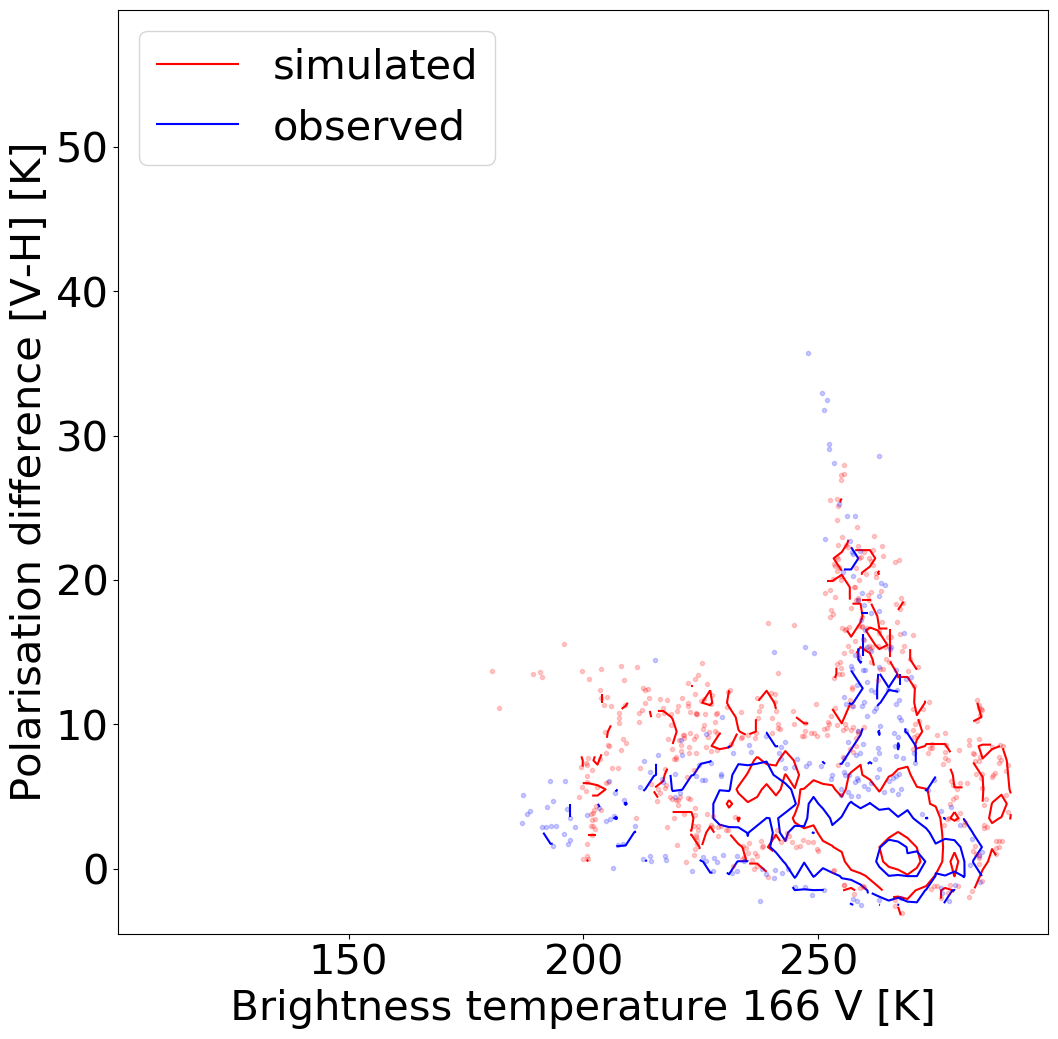
\includegraphics[height =35mm]{Figures/hist2d_gmi_45-60_land.png}
	\end{subfigure}
	\begin{subfigure}{.24\textwidth}
		\caption{Water}
		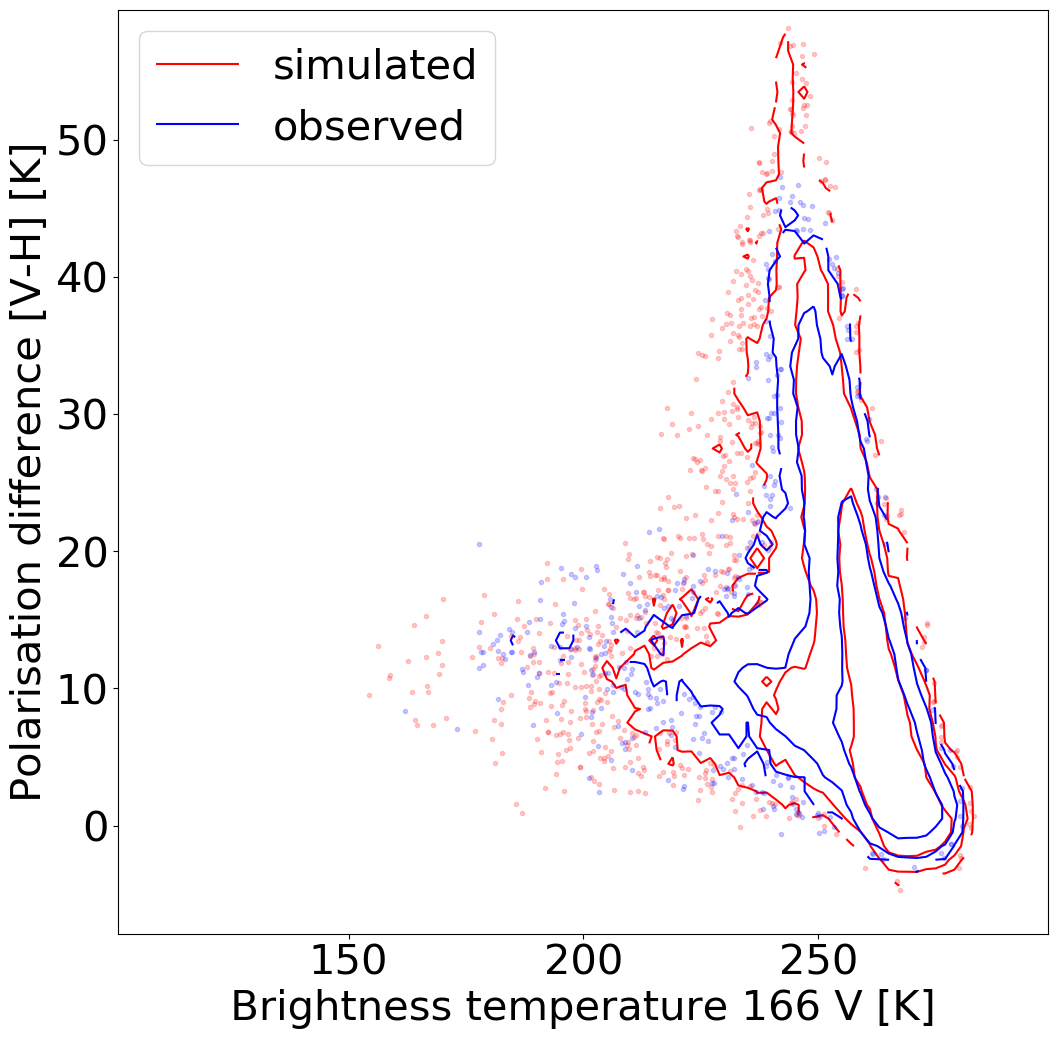
\includegraphics[height = 35mm]{Figures/hist2d_gmi_45-60_sea.png}
	\end{subfigure}
	\begin{subfigure}{.24\textwidth}
	\caption{Snow}
	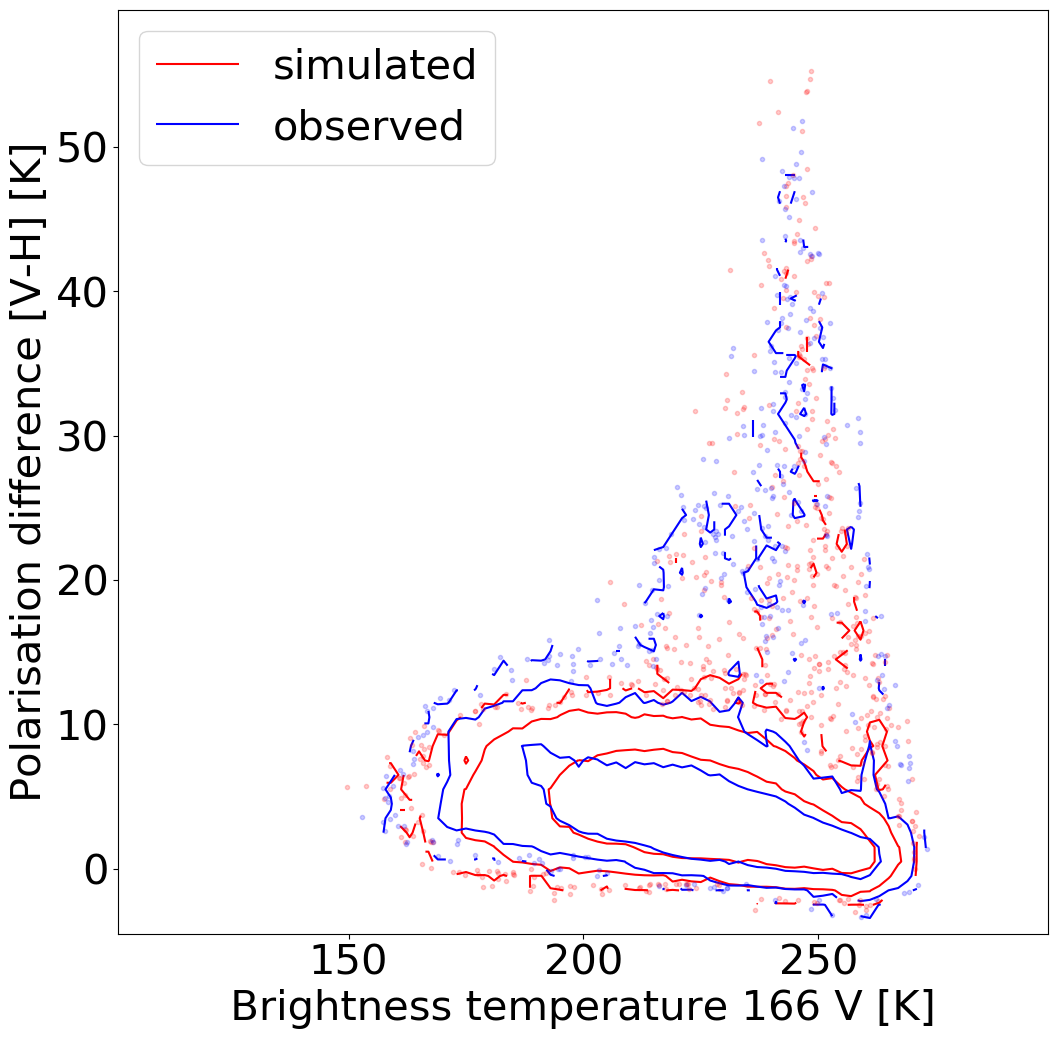
\includegraphics[height = 35mm]{Figures/hist2d_gmi_45-60_snow.png}
\end{subfigure}
\begin{subfigure}{.24\textwidth}
	\caption{ Sea-ice}
	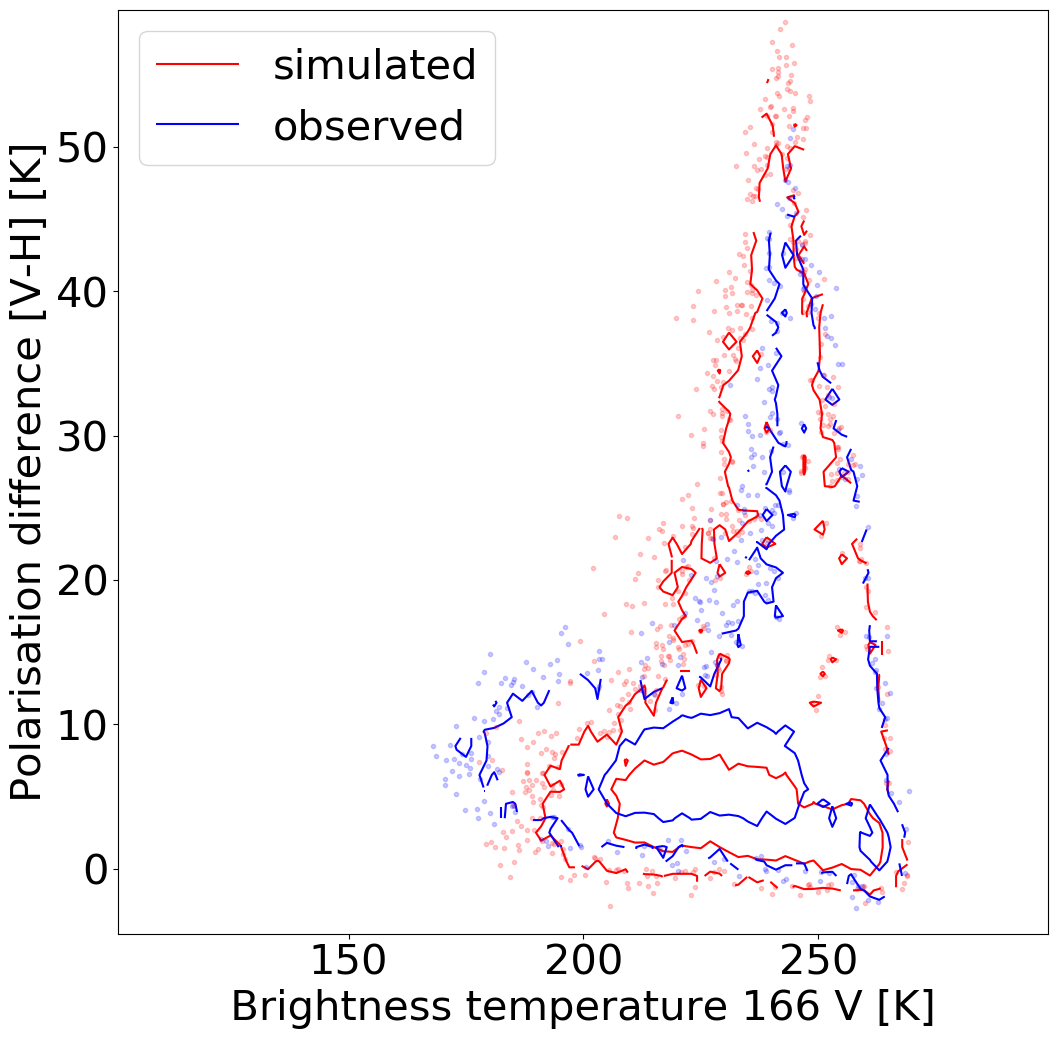
\includegraphics[height = 35mm]{Figures/hist2d_gmi_highlat_sea-ice.png}
\end{subfigure}
	\caption{Two-dimensional PDFs for the TB and PD for GMI 166\,GHz frequency. Figures (a)-(d) are for land, water, snow and sea-ice surface types respectively. The simulated GMI data is from Jan 2009, while GMI measurements are from Jan 2020.}
	\label{fig:histogram_2d}
\end{figure*}

In order to verify that the data in the training database covers the actual measurement space, the measured and simulated TB from GMI are compared statistically. Figure~\ref{fig:histogram_2d} shows the polarisation difference (PD) and TB histograms from 166 GHz for different surface types. The PD is defined as the difference between vertical and horizontal polarisations. The effect of including particle orientation using the scheme of \citet{baralakas:intro:21} indeed looks promising to mimic the effect of hydrometeor interaction.
Over both sea-ice and snow, the PDs are mostly positive as a consequence of hydrometeor scattering, and the negative PDs arise from noise in clear-sky measurements. For all surface types, the variability of our simulations is higher than the GMI measurements, indicating that the simulations can cover all possible range of conditions. This is an important result as we cannot expect the retrieval to provide a complete picture if the training database covers the measurement range partially.

\subsubsection{Retrievals}
\label{sec:preliminary_results}
\begin{figure*}[t]
	\centering
	\begin{subfigure}{.54\textwidth}
		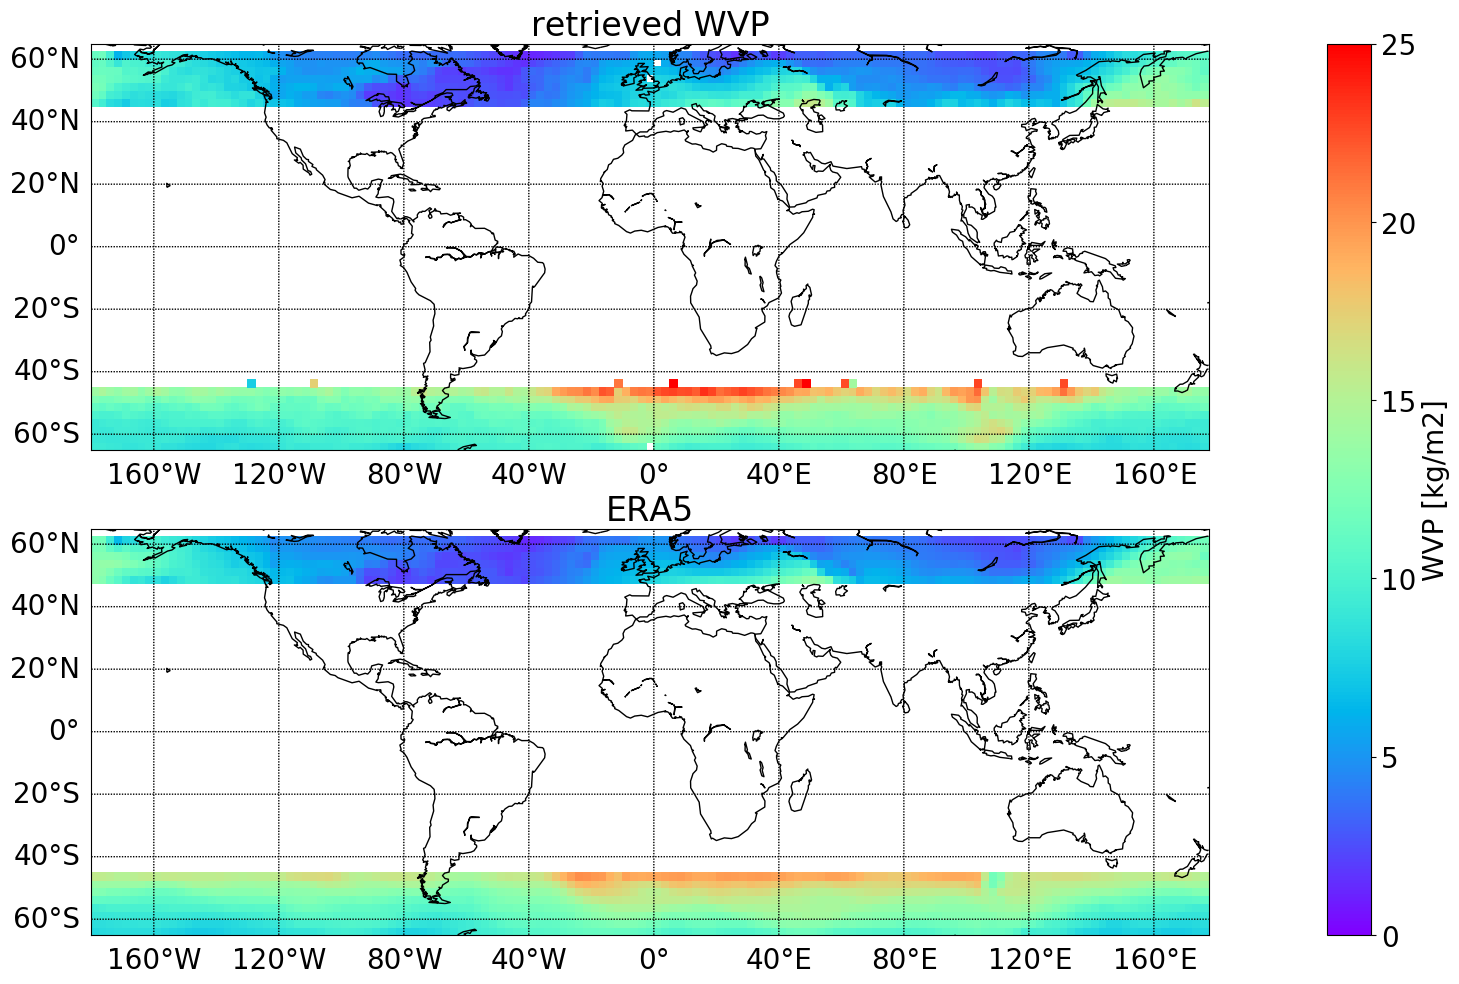
\includegraphics[height = 55mm]{Figures/WVP_spatial_jan2020.png}
	\end{subfigure}
	\begin{subfigure}{.34\textwidth}
	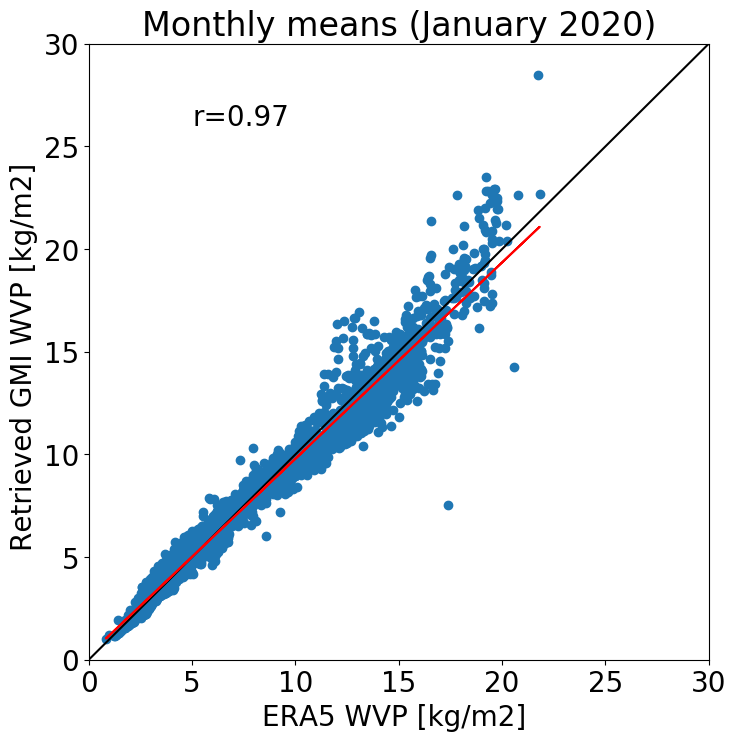
\includegraphics[height = 50mm]{Figures/WVP_scatter_monthlymean.png} 
	\end{subfigure}
	\caption{The spatial distributions (left) of monthly means estimated from retrieved WVP and ERA5 WVP. The data is for January 2020. The corresponding scatter between the two datasets is shown on the right. The red line is the line of best fit, while the black indicates the perfect fit.}
	\label{fig:WVP_retrievals}
\end{figure*}


The QRNN algorithm described in sect.~\ref{sec:qrnn} is applied to measured TB from GMI frequencies: 166 V\,GHz, 166 H\,GHz, 183$\pm$3\,GHz and 183$\pm$7\,GHz, to retrieve the corresponding WVPs. Two-metre temperature, latitude and surface type are also provided as auxiliary information. No data filtering is applied. In order to compare the retrieved WVP with ERA5 total column water vapour (TCWV), the retrievals are re-gridded to 2.5$^{\circ}$ resolution. A comparison of the near global maps (between 45$^\circ$ - 65$^\circ$) of monthly means from both datasets is displayed in fig~\ref{fig:WVP_retrievals}. The two spatial distributions largely agree with each other except for few high WVP values in the southern hemisphere. The correlation between the two datasets is 0.97. Over the southern hemisphere, the saturation of high-frequency channels over high humidity regions could be responsible for the inaccurate retrievals.

\subsubsection{Sea-ice classification using SARS}
\todo{from Leif}

\subsection{Work Flow}
\label{sec:wp}

\subsubsection*{WP 1: Basic atmospheric scenarios}
%
\begin{figure*}[t]
	\centering
	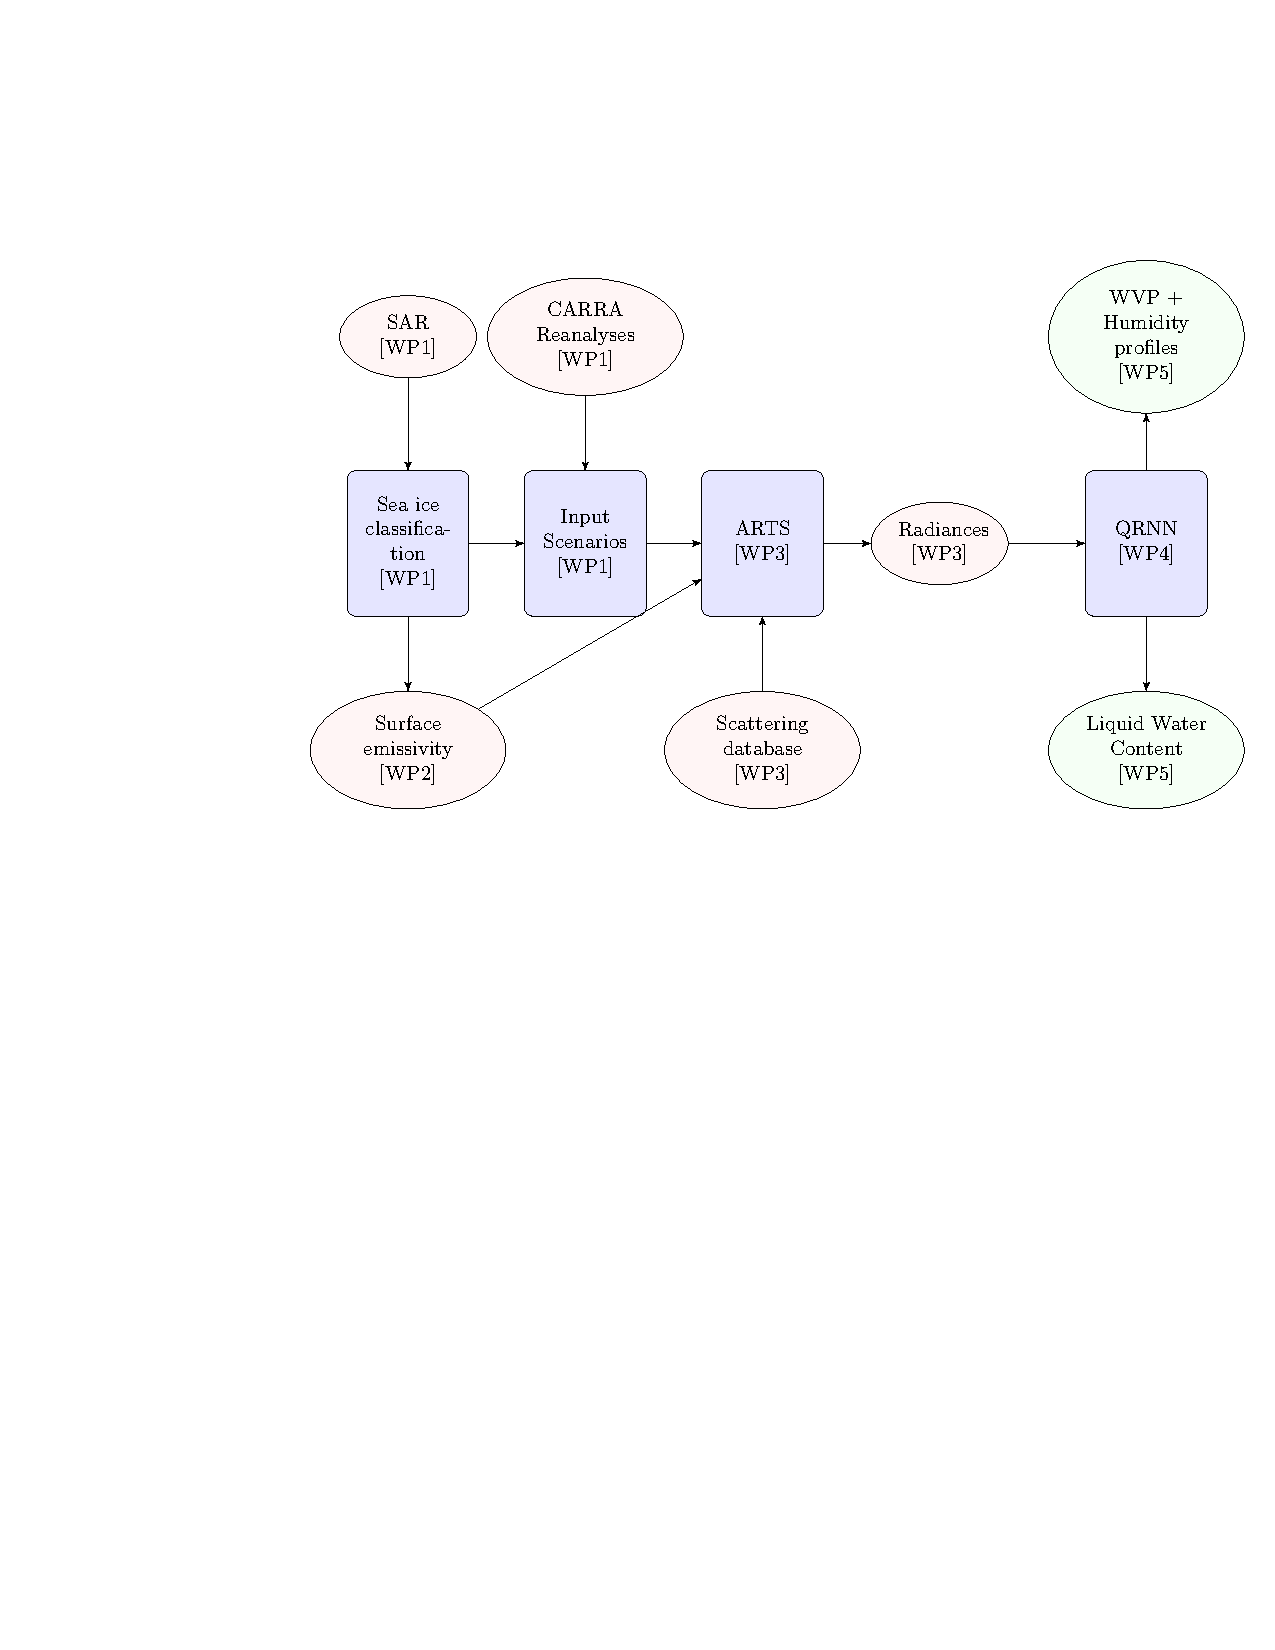
\includegraphics[trim=140 370 40 125,clip,height = 60mm]{flowchart.pdf} 
	\caption{Flowchart displaying schema of the proposed retrieval system.}
	\label{fig:flowchart}
\end{figure*}
\label{sec:emissivity}
The inputs to the forward model can be based on either atmospheric models providing a sufficiently detailed description of hydrometeors or on observations as far as possible \citep{ekelund:using:20}. In this study, we shall use the former approach and use reanalyses from HARMONIE-AROME to create a database of the atmospheric cases. HARMONIE-AROME does not cover all Arctic regions, so if needed, reanalyses from ERA5 could be included. If found necessary, we could also explore the latter approach and apply our own microphysical assumptions. Furthermore, the high-resolution SAR imagery would be employed to characterize the sea-ice/open waters. The fine spatial resolution of SAR would facilitate better mapping of inhomogeneous surface types and thus reduce errors with modelling ocean-atmosphere heat flux in mixed surface types such as coastlines and polynyas. To our best knowledge, this would be the first instance where such high-resolution information would be used. Also see fig.~\ref{fig:flowchart} for the flowchart.
The output of this work package would be a broad set of 3D atmospheric scenarios to be used as input to the radiative transfer simulations.

\subsubsection*{WP 2 : Emissivity model}
%
\label{sec:emissivity}
An important step to accomplish this task is the estimation of the surface emissivity spectra over a multitude of surface types. As a first step, we would consider using existing studies to extend the snow-emissivity model (see sect.~\ref{sec:radiative_transfer}) to lower frequencies such as 89\,GHz and 50\,GHz. Such an empirical model would be easy to fine-tune by comparing results from pure forward modelling. However, the final aim would be to use the Optimal Estimation method (OEM) on the high-resolution scenes to extract microwave emissivity spectra from TB. We would consider joint retrievals of emissivity spectra over all frequencies. The basic idea of joint retrievals is to find a set of emissivity estimates for all considered frequencies which would simultaneously give TB closest to the measurements. The synergy between such retrievals is especially useful to understand the emissivity correlations between frequencies. Thus making it more viable from an assimilation perspective. Retrievals in this WP would be made assuming both specular and lambertian reflection. The differences between the two are immaterial for conical instruments, but for cross-track instruments the realistic situations could be considered as a combinations of two. Tests would be made to judge exactly what combination works best for various surface types. 

%ARTS would be used for OEM retrievals.

The output of this work package would be measures of high resolution all-weather sea-ice emissivities at different frequencies. 
	
\subsubsection*{WP 3 : Database creation and post-processing}
%
\label{sec:database}	
This WP would cover the initiation and execution of the batch radiative transfer calculations (with ARTS). Initially, some time will be needed to implement the scripts needed for the basic calculations, to add jobs to the calculation cluster, and post-processing. As a start, only conical scanners would be simulated, and later extension to cross-track scanners should be straightforward. For the latter, a number of scan angles, between nadir and swath edge, will be covered.

For both types of scanners, the overlapping antenna footprint of all frequencies will be explicitly simulated so that it is feasible to retrieve parameters at a finer scale than individual antenna beams. To generate the antenna pattern at the desired frequency, a number of pencil beam radiative transfer calculations will be performed to incorporate both along-track and across-track sampling. Bias adjustments to the forward model simulations would also be made as a post-processing step. For forward modelling to accurately represent the satellite measurements, bias adjustments as calculated by ECMWF would be applied. Sensor calibration and its relative agreement with the forward model are vital for the success of the retrieval database. 
The WP output shall be batches of simulated radiances.

\subsubsection*{WP 4 : Retrieval setup}
%
\label{sec:setup}
The use of the retrieval database shall be made without introducing any re-mapping between the different footprint sizes. All footprints inside a region would be used as input, and the database generation will mimic this. This approach will make much better use of the spatial information provided by the overlap of instrument footprints. The target resolution would not be compromised and retrievals can be made at the highest possible resolution while preserving the information at their native resolution. This has been demonstrated using 2DVAR in \citet{duncan:onthe:19}. But here we shall aim to achieve the same purpose by using QRNN. In fact, by doing this by a database (and not 2DVAR) we are not restricted to describe spatial correlations by covariance matrices and the QRNN version should be even more advantageous.

The package for QRNN is already available as a part of the Typhon software package \citep{lemke:2020:typhon}. The implementation of the retrieval algorithm shall be relatively straightforward but the challenge would be to find the best performing neural-network architecture so as to achieve the best model performance. Besides, it would also be important to test the sensitivity of various auxiliary data to the retrieval performance. In order to run the retrievals, we shall make use of the Chalmers central computational cluster (C3SE).


\subsubsection*{WP 5 : Retrievals}
%
\label{sec:retrievals}
%
In this WP, as a first step, we will extend our preliminary results for WVP (see sect.~\ref{sec:preliminary_results}) to include regions north of 65$^\circ$, using SSMIS.  An extension to lower frequencies such as  89\,GHz and temperature sounding channels around 50\,GHz will be tested. Including the latter can also be beneficial to resolve the low-level cloudiness and hence improve the humidity profiles. Infact, the estimates of LWC and WVP are not completely independent. The synergies between the two quantities can be exploited to correct the estimates for each other. For LWC over sea-ice, the combination 89+150\,GHz have been suggested by \citet{laue:2007:poten} to cancel out the effect of emissivities. Inclusion of 22\,GHz and 37\,GHz to increase sensitivity to high humidity regions could also be considered, though on a lower priority. These channels are more important over open-waters than sea-ice regions. Later, the best channel combinations will also be used to estimate the humidity profiles. The ultimate goal is to include sufficient channels such that the full information content of tropospheric water is preserved. Extension to cross-track scanners shall also be made. This will require slightly more work. A larger database covering the various incidence angles will be necessary, but we would focus only on the central part of the swath, and avoid working with very large footprints towards the edge of the swath. 
%The pivotal part of these retrievals would be using ML on the overlapping footprints to extract the hidden information without any explicit treatment.

We will start the test retrievals in parallel to database creation so that early feedback on any issues could be made. QRNN is versatile to allow extension to include additional input channels or auxiliary data but the main task will be to analyse the results. During the development phase evaluation, (see sect.~\ref{sec:evaluation}) of the retrievals with existing retrieval products will be made to identify the areas requiring improvement.

The output of this WP would be one or more retrieval databases for WVP, LWC and humidity profiles.

\subsubsection*{WP 6: Evaluation and dissemination}
%
\label{sec:evaluation}
The evaluation part shall go hand-in-hand with the retreival WP. The main tasks of this work package are to evaluate the quality of the retrievals, understand the discrepancies, and pave way for their optimal use. Since in this project we aim to solve the retrieval issues associated with the ever complex and changing surface characteristics of sea-ice, a detailed assessment would be expected to improve the applicability and future retrieval algorithms. In this work package a thorough investigation with the available \textit{in-situ} data, satellite products and reanalysis would be made. Firstly, direct comparisons with radio-soundings or data from flight campaigns would be used to estimate the accuracy of the product and reveal the uncertainties on finer scales.  Statistical comparisons with other microwave and IR based humidity products  will also be made. Time series of daily and monthly means, and the probability distribution functions (PDFs) of the retrievals would be analysed. Here it would also be important to analyse the accuracy over seasons and different surface types. 

The dissemination of the retrieved dataset will be through conferences and journal articles. The assessment of how well the produced dataset answers the needs of NWP communities will also be addressed through collaborations with ECMWF and SMHI. Patrick Eriksson has been one of the leading contributors to the preparation of AWS and would also be involved in a Nordic weather study with SMHI around AWS. Furthermore, the contact with ECMWF is strengthened by the fact that Patrick Eriksson has been appointed ECMWF fellow. Contact with David Duncan at ECMWF would also be continued. 

\subsubsection*{WP 7 : Additional Retrievals}
%
\label{sec:other_retrievals}

Secondary products which would be considered include snow and sea-ice concentrations.  

\todo{snow}

The high-resolution emissivity retrievals can be additionally post-processed to generate estimates of sea-ice concentration. The post-processing simply involves matching the 1D-VAR emissivity estimates over sea-ice to a pre-computed catalog of mean emissivity spectra. 

%Infact, validation of the SIC against other available products like MiRS (Microwave Integrated Retrieval System) based operational cyrogenic products  (\url{https://www.star.nesdis.noaa.gov/mirs/highresolutionv.php}) can also serve as an indirect validation of the emissivity retrievals.

\subsection{Impact and social benefits}
%
\label{sec:impact}
Arctic amplification is garnering rapid interest, thus increasing the need to provide better understanding of weather, environmental and climate processes in the polar regions. Towards improving our ability at making reliable forecasts efforts, amplifying the usage of satellite derived polar products in numerical models is crucial. In other ways, it also has implications on mid-latitude weather forecasts. We propose that the proposed standalone retrievals of Arctic water shall improve the ingestion of satellite data than it is being done now. Additionally, high resolution emissivity information would also be an important result which could assimilation of microwave observations over polar regions. This aspect shall be covered in association and feedback from numerical modelling community at SMHI and ECMWF (see sect.~\ref{sec:evaluation}).

As a society, the anthropogenic climate change over poles has economic and political implications. Increasing economic activity through Arctic navigation also requires substantial efforts to be conducted in a safe manner. Reducing uncertainties in the weather forecast being an important component. 

%LWC over polar regions are major contributors to uncertainty in retrievals of sea ice concentration by passive microwave radiometry.
 
\subsection{Risk Assessment}
%
\label{sec:risk}
The overall risk around this project is considered to be low. The project in continuation or on similar lines as the other projects the group is working on.

 There is some speculation around the usage of low frequencies like 22\,GHz and 37\,GHz considering their large footprint size. \todo{incomplete...} 

\section{Collaborations}

ECMWF and SMHI ?
%In order to receive feedback on the retrieval database, we would closely collaborate with group working on WVP retrievals at University of Bremen to cover the analysis and validation aspects. Additionally, a contact with the group of Prof. Susanne Crewell could also be useful for validation purposes. Their group is operating the MiRaC airborne sensor (a combined radar and radiometer) during polar flights (Mech et al., 2019).

\section{Staff situation/ Roles and responsibilities?}
\label{sec:staff}
%
Inderpreet Kaur started as a postdoctoral researcher in the division during March 2020.  She is presently working with retrieval of atmospheric ice using microwave instruments. During the project period, she shall spend 80\,\% of her time the project. Patrick Eriksson is a professor and has main expertise in atmospheric radiative transfer and retrieval methods. He will spend 5\% of his time on this project and contribute to all WPs. Luisa Ickes is an Assistant Professor, and has special research interests are the Arctic region and clouds in general. She will provide expertise in cloud physics, both when generating training data and evaluating retrievals (WPs 5, 6). Leif Eriksson is group leader for the research group Radar Remote Sensing. His research is aimed at development of methods to make measurements of land and ocean with radar data. In this project, his expertise is sought on the use of SAR data in the project. He will mainly contribute to WP 1 and WP 7. 

\section{Satellite data}
%
All satellite data of concern, in this project, is publicly available. 

{\footnotesize
	\bibliography{j_abbr,refs_pe1,references}
}
\end{document}
